\chapter{Deployment}
\label{chap:deployment}

\section{Containerization and s6-overlay supervision}
\label{sec:s6-overlay}

Some RAM-USB services must run several independent processes in the same container and
therefore need a supervisor that starts them in the right order and restarts them when they go down.
The one used by RAM-USB is \texttt{s6-overlay} \cite{s6-overlay-github}.
Each supervised process is a directory under \texttt{s6-rc.d/}, declared as type \texttt{longrun};
its dependencies are files inside a \texttt{dependencies.d/} subdirectory, one for each process that
must be started: if, for example, process A must wait for process B to be ready,
\texttt{A/dependencies.d/} contains an empty file named \texttt{B}.
The startup order therefore arises from a graph declared between directories.
Storage-Service is the most complex case: the same Docker container is shared by four processes
\cite{ramusb-code-storage-s6-tree}: \texttt{tailscaled}, the actual mesh client; \texttt{sshd}, the
SFTP server (\autoref{chap:storage}); \texttt{identity-provisioner}, which keeps the X.509 certificate
for mTLS up to date; and the Go binary of Storage-Service itself, which exposes the internal HTTP API.
Each \texttt{longrun} process also has a \texttt{run} file and a \texttt{finish} file. The first is the
script that launches the actual binary \cite{ramusb-code-storage-s6-tree}.
If that process terminates, the supervisor relaunches it from scratch;
the second is optional and is used to delay the relaunch by a few seconds, so as to prevent an irreversible
startup error from turning into a continuous crash loop.

Not all services, however, need this complexity. Entry-Hub, for example, does not supervise
any secondary process: its membership in the mesh lives in a separate Docker sidecar,
\texttt{entry-hub-mesh}, which shares its network namespace. The following section explains how
this difference is tied to the choice of each service's base image.

\section{Why not all containers are distroless}
\label{sec:distroless}

A distroless image \cite{distroless-github} has neither a shell nor a package manager, which substantially reduces
the number of known critical vulnerabilities in containers \cite{wager2024distroless}.
A supervisor such as \texttt{s6-overlay}, however, needs a shell for its own startup scripts.
Any service that must run more than a single Go binary therefore cannot be distroless.
Consequently, the only distroless service is Entry-Hub \cite{ramusb-code-dockerfile-entry-hub}, while
the other six use \texttt{debian:bookworm-slim} or \texttt{alpine}, as shown in
\autoref{tab:immagini-base}.

\begin{table}[H]
\centering
\caption{Base image of each service and the processes sharing its container.}
\label{tab:immagini-base}
\begin{tabular}{@{}l p{\dimexpr0.3\linewidth\relax} p{\dimexpr0.38\linewidth\relax}@{}}
\hline
\textbf{Service} & \textbf{Base image} & \textbf{Shares the container with} \\
\hline
Entry-Hub & distroless & none (mesh in a separate sidecar) \\
Security-Switch & debian:bookworm-slim & \texttt{tailscaled} \\
Network-Manager & debian:bookworm-slim & \texttt{tailscaled} \\
Storage-Service & debian:bookworm-slim & \texttt{tailscaled}, \texttt{identity-provisioner}, \texttt{sshd} \\
Database-Vault & \texttt{postgres:17} (Debian) & \texttt{tailscaled}, \texttt{postgres} \\
Metrics-Collector & \texttt{timescaledb} (Alpine) & \texttt{tailscaled}, \texttt{timescaledb} \\
Certificate-Authority & \texttt{step-ca} (Alpine) & \texttt{step-ca} (mesh in a separate sidecar) \\
\hline
\end{tabular}
\end{table}

Extending distroless to more services or choosing distributions other than those listed in
\autoref{tab:immagini-base} is an issue that has not yet been addressed.

\section{Local Docker vs Proxmox VE: two levels of isolation}
\label{sec:docker-vs-proxmox}

It would be natural to think of Docker and Proxmox VE \cite{proxmox-ve} as two alternatives for the same
isolation need. In reality they operate at two different levels. Docker is a containerization engine:
it isolates a process at the operating system level, sharing the kernel with the host, so that each container
sees its own filesystem, its own network, and its own process tree without the cost of a second
kernel \cite{docker-overview}. It thus guarantees portability across operating systems and per-service
isolation, identical in development and in production.

Proxmox instead adds, on top of each Docker container, the isolation boundary of a KVM virtual machine,
with its own kernel, or, alternatively, that of an LXC system container, lighter but sharing the kernel
with the host. Each service therefore runs inside its own Docker container, but that
Docker container in turn runs inside its KVM virtual machine or inside its LXC container.
Choosing Proxmox also brings another advantage: it paves the way for live migration of the KVMs
and, with more nodes, for high availability.

Storage-Service, Database-Vault, and Network-Manager are assigned to KVM guests, while the remaining
services are assigned to unprivileged LXC containers, in which the container's root user is therefore mapped
to a non-root user of the host.
Entry-Hub and Headscale stay outside Proxmox entirely, each on its own dedicated public VPS, for the
reasons explained in \autoref{chap:rete}.

The choice between KVM and LXC depends, for almost all services, on the level of isolation they require.
LXC containers share the kernel with the host system, so they are not fully isolated, but
they need very few resources, so the host can run several of them at the same time. For this
reason they are the default choice.
The services that hold user data, manage network policies, and store backups need
greater isolation, because their compromise could cause irreparable damage.
Storage-Service also needs to run \texttt{setuid} and \texttt{chroot} to isolate POSIX
users (\autoref{sec:isolamento}): doing so inside an LXC container, itself already a namespace,
would add a second level of UID mapping. A KVM avoids stacking
two isolation mechanisms that do not compose cleanly \cite{ramusb-proxmox-storage-service}.

\section{Distributed topology}
\label{sec:topologia-distribuita}

The repository contains eleven separate Compose files under \texttt{deployments/compose/}
\cite{ramusb-code-compose-tree}. Ten correspond to the internal components
(\autoref{chap:architettura}); the eleventh, \texttt{tailscale-test.yml}, supports testing.
Containerization of the client is instead left to future work.
Each component's file remains independent of the others because every service is designed to be
started, stopped, or moved to a different Proxmox node, into a different KVM guest or LXC container.

\autoref{fig:architecture-deployment} summarizes the production topology.

\begin{figure}[H]
\centering
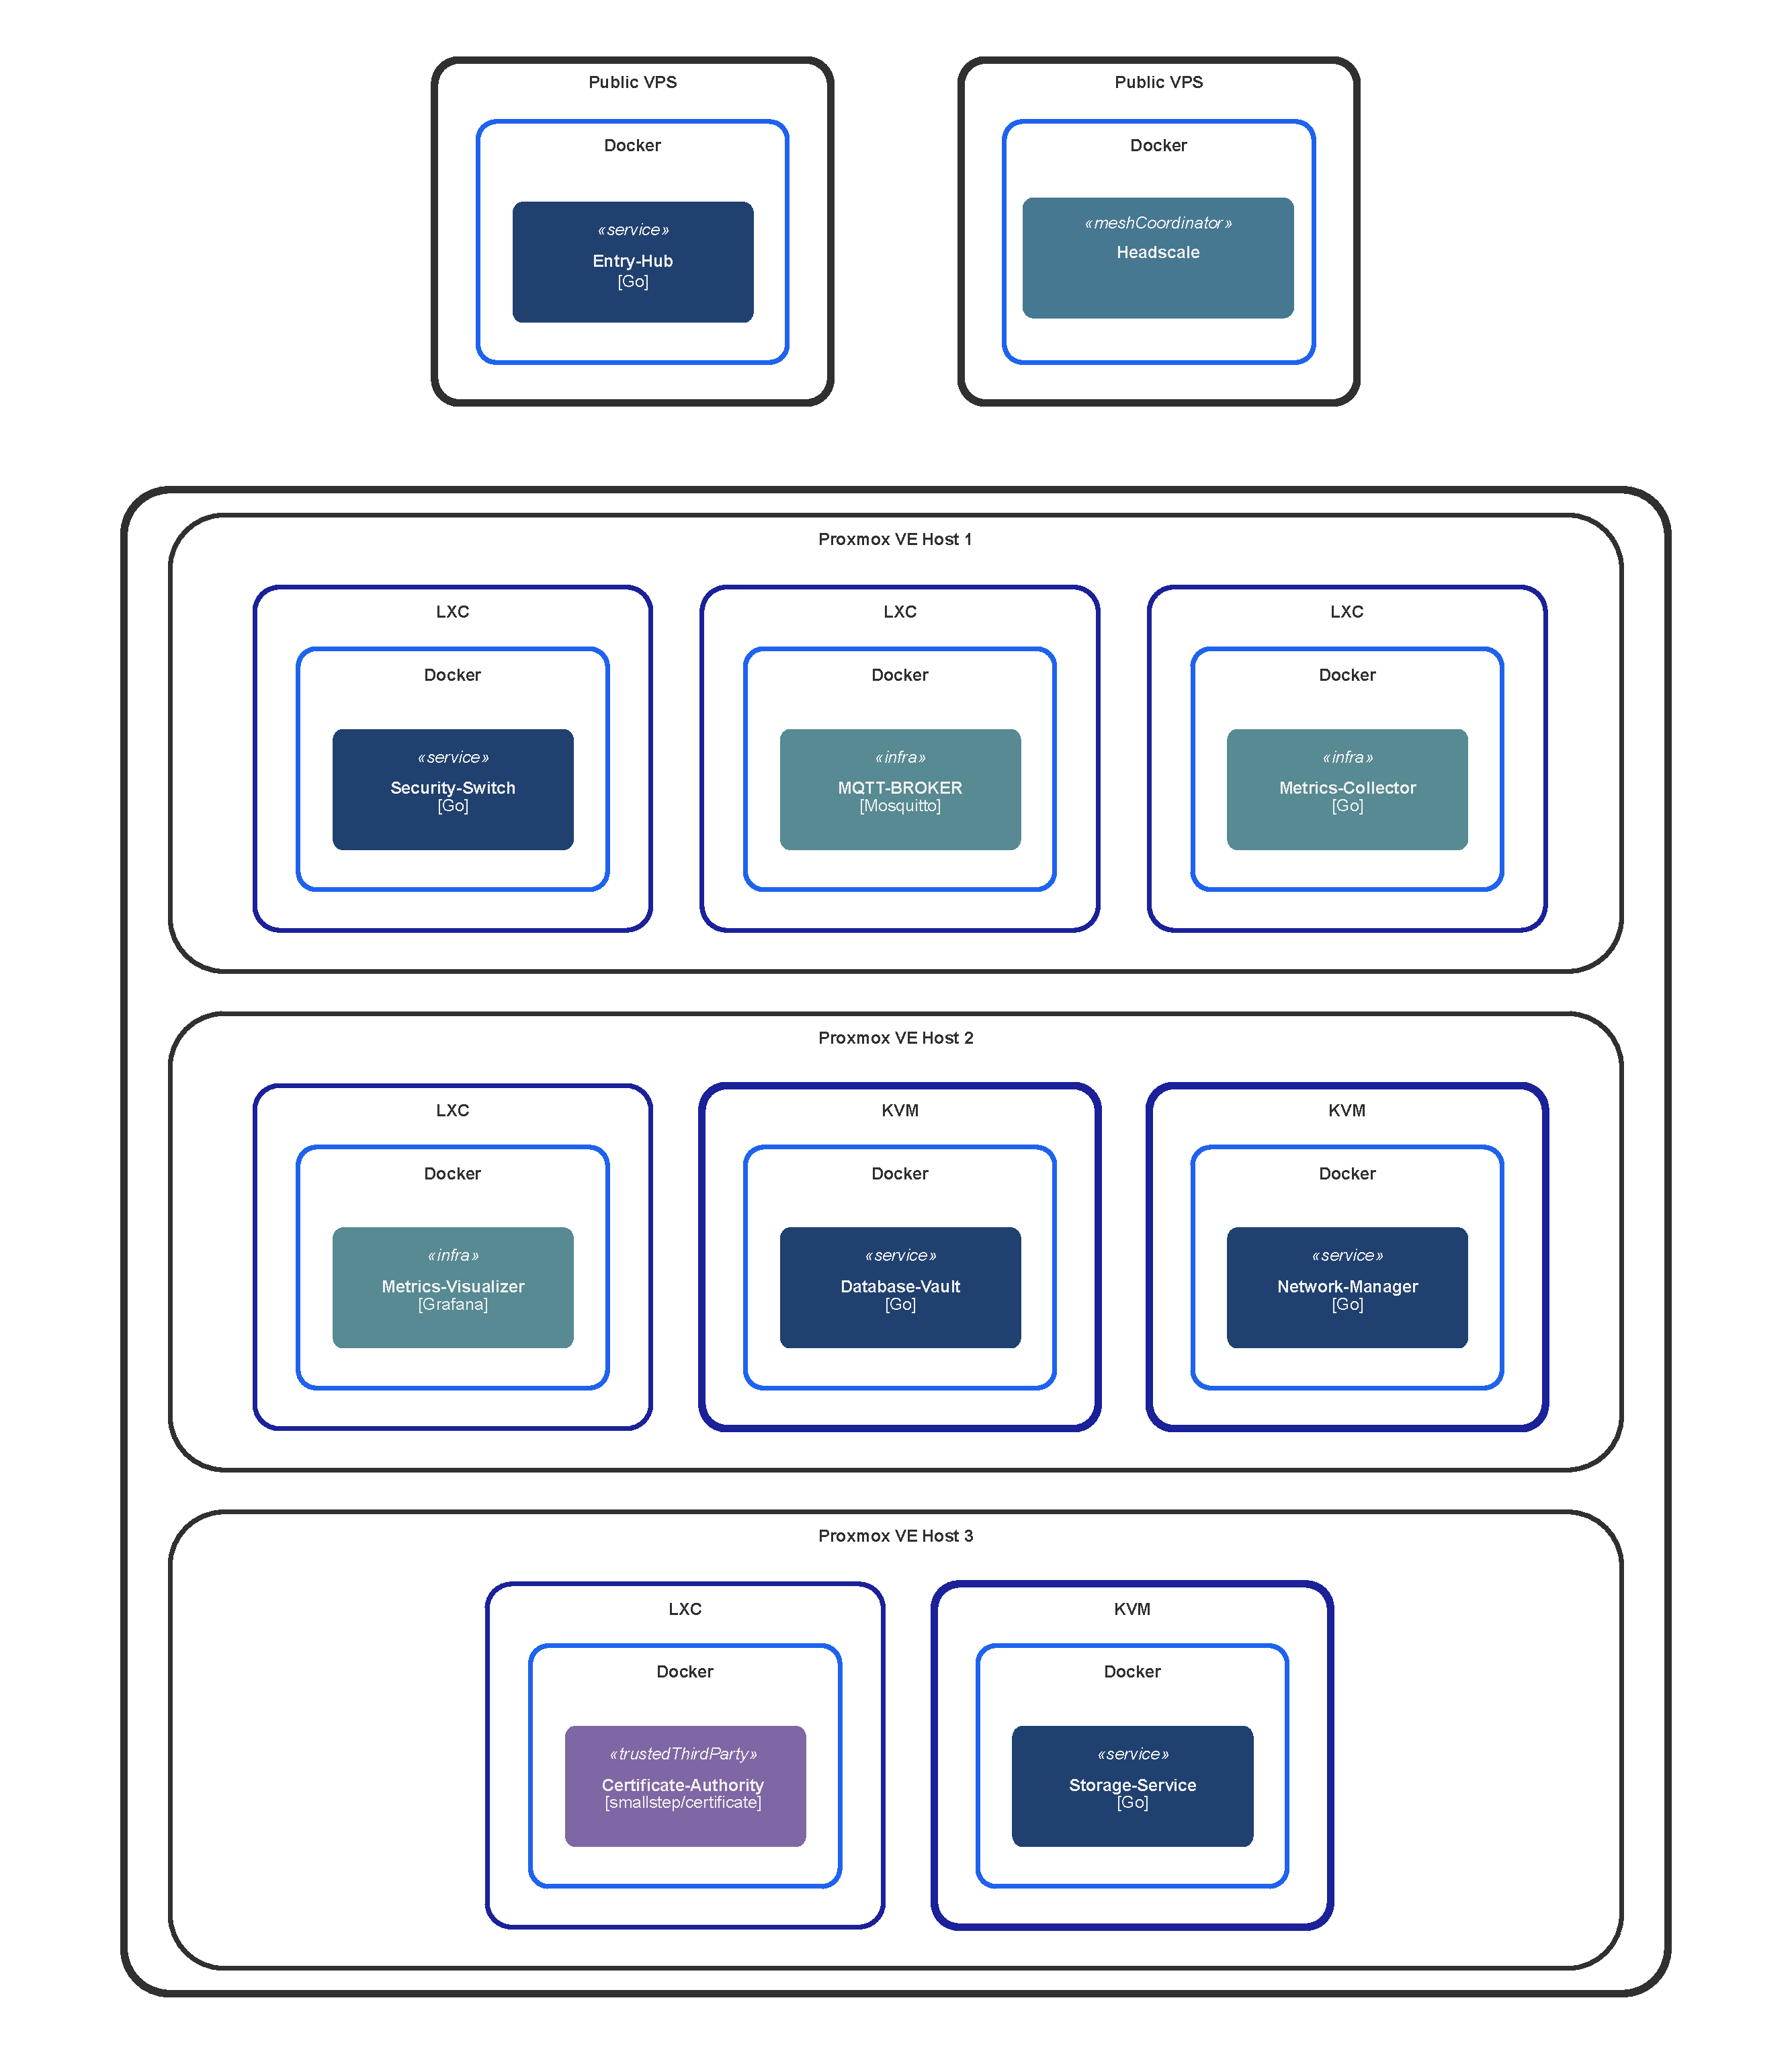
\includegraphics[width=0.95\textwidth]{figures/02-architecture-deployment.pdf}
\caption{Target production topology.}
\label{fig:architecture-deployment}
\end{figure}

\section{High availability and resilience: current state and limitations}
\label{sec:ha-limiti}

The service remains available to users only as long as the components that take part
in a request's path remain available.

The number of available physical nodes determines how much resilience and fault tolerance RAM-USB
can achieve: each added node unlocks one more property.

With a single physical node, \texttt{s6-overlay} supervision restarts a crashed process inside
a Docker container (\autoref{sec:s6-overlay}), but does not cover the unavailability of the physical node the
service runs on. Moreover, the most that can be achieved is local disk redundancy, for example with
RAID-10.

A second node unlocks zero-downtime migration of KVMs from one node to another, to balance the
load or free one up for maintenance \cite{proxmox-qm-migration}.
LXC containers, on the other hand, cannot be live-migrated, only restarted elsewhere \cite{proxmox-pct-migration}.

With at least three nodes and storage replicated with Ceph, the system becomes a hyperconverged cluster,
able to offer automatic recovery after the failure of a physical node, in addition to the planned
relocation of a healthy one.

The nodes, however, must be on the same low-latency network in order to cooperate, since the Proxmox cluster
stack requires a latency below 5 ms between all nodes \cite{proxmox-cluster-manager} to operate
stably.

Even with the best fiber available, two nodes far apart cannot reach such a low
latency. Extending the Proxmox backend to multiple sites would require a different mechanism, not yet planned.
At present, hyperconvergence and geo-distribution are mutually exclusive.
Achieving both at the same time remains an open problem outside the scope of RAM-USB.
